% !TEX root =big-fish.tex
\chapter{Movement design}
The goal of this chapter is to explain the raw motion design, based on which the collision prediction and avoidance algorithms will be established.\\

The velocity of a fish is meant to represent its site's response time; in order to clearly notice it, circular trajectories have been chosen to define the nature of the movement.\\

However the trajectory might change depending on a fish's state. For this reason, a fish aggregates the motion logic to its state thereby applying the strategy design pattern.\\

Note that the rest of this section assumes the reader to be familiar with Euler rotations which are a corner stone in 3D development. Figure ~\ref{fig:euler-rotations} can help understanding the rotations mechanism; it illustrates step by step the application of Euler rotations given ZXY as Euler order: 

\begin{figure}[H]
   \centering
   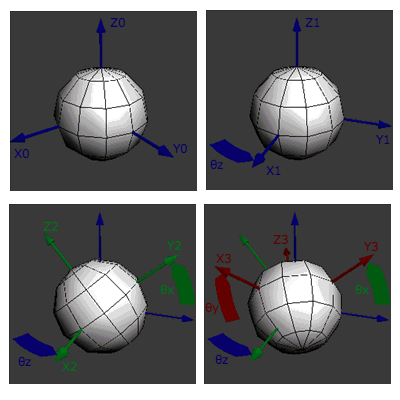
\includegraphics[scale=0.65]{figures/euler.png}
   \caption{Euler Rotations}
   \label{fig:euler-rotations}
\end{figure}

The 4 snapshots illustrated in figure ~\ref{fig:euler-rotations} represent:
\begin{itemize}
\item The axis initial states before any rotation gets applied.
\item The axis after applying a rotation $\theta _{z} $ around the Z axis.
\item The axis after applying $\theta _{z}$ followed by $\theta _{x}$.
\item The axis after applying $\theta _{z}$ followed by $\theta _{x}$ followed by $\theta _{y}$.
\end{itemize}

The rest of the chapter describes the different states a fish might go through.

\section{Swimming state:}
\label{subsec:swimmingstate}

The swimming state is where a fish spends most of its time. Even when a particular event triggers a change of state, as soon as the cause disappears, the fish immediately returns to the swimming state.\\

The movement nature of the swimming state is circular; the radius and the center of the circle is common to all the fishes in the scene. This means that all fishes are swimming within the same sphere surface. However to create diversity in the movement, the planes holding each fish's trajectory are different. Considering YXZ as the Euler rotation order, all the trajectories' planes have the same $\theta _{x}$ rotation defined as a constant to represent the planes' inclination, whereas $\theta _{y}$ rotations are different per fish. The difference is obtained by adding a $\Delta \varphi$ deviation whenever a new fish gets loaded.\\

A plane's orthonormal coordinate system is defined by two orthonormal axis and a center. The center is common to all the trajectories' planes i.e. the center of the scene, whereas calculating the axis coordinates required some mathematical analysis that led to the following results:\\

Let $\overrightarrow{X_{1}}$, $\overrightarrow{X_{2}}$, $\overrightarrow{X_{3}}$ be the rotated axis, where $X_{1}X_{2}X_{3}$ denotes Euler order, and let $\theta_{1}$, $\theta_{2}$ and $\theta_{3}$ be the corresponding Euler rotations. If we consider ($\overrightarrow{x_{1}}$, $\overrightarrow{x_{2}}$, $\overrightarrow{x_{3}}$) as the reference coordinate system, $\overrightarrow{X_{1}}$, $\overrightarrow{X_{2}}$ and $\overrightarrow{X_{3}}$ coordinates can be obtained by applying the following formula:
\[
\begin{array}{lllll}
\overrightarrow{X_{1}} = \begin{pmatrix}
\cos{\theta_{2}}  \cos{\theta_{3}} \\
\sin{\theta_{3}}  \cos{\theta_{1}} + \cos{\theta_{3}}  \sin{\theta_{2}}  \sin{\theta_{1}}\\
\sin{\theta_{3}}  \sin{\theta_{1}} - \cos{\theta_{3}}  \sin{\theta_{2}}  \cos{\theta_{1}}
\end{pmatrix}_{(\overrightarrow{x_{1}}, \overrightarrow{x_{2}}, \overrightarrow{x_{3}})}\\ \\

\overrightarrow{X_{2}} = \begin{pmatrix}
-\sin{\theta_{3}}  \cos{\theta_{2}} \\
\cos{\theta_{3}}  \cos{\theta_{1}} - \sin{\theta_{3}}  \sin{\theta_{2}}  \sin{\theta_{1}}\\
\cos{\theta_{3}}  \sin{\theta_{1}} + \sin{\theta_{3}}  \sin{\theta_{2}}  \cos{\theta_{1}}
\end{pmatrix}_{(\overrightarrow{x_{1}}, \overrightarrow{x_{2}}, \overrightarrow{x_{3}})}\\ \\

\overrightarrow{X_{3}} = \begin{pmatrix}
\sin{\theta_{2}}\\
-\cos{\theta_{2}}  \sin{\theta_{1}}\\
\cos{\theta_{2}}  \cos{\theta_{1}}
\end{pmatrix}_{(\overrightarrow{x_{1}}, \overrightarrow{x_{2}}, \overrightarrow{x_{3}})}
\end{array}
\]\\
Mapping the indices to the corresponding axis will convert the coordinates relatively to the reference coordinate system, thus giving the new rotated axis ($\overrightarrow{X}$, $\overrightarrow{Y}$, $\overrightarrow{Z}$).\\

\subsubsection{Example}
If we consider YXZ for instance as the Euler rotation order, ($\overrightarrow{X_{1}}$, $\overrightarrow{X_{2}}$, $\overrightarrow{X_{3}}$) would map to ($\overrightarrow{Y}$, $\overrightarrow{X}$, $\overrightarrow{Z}$), and ($\overrightarrow{x_{1}}$, $\overrightarrow{x_{2}}$, $\overrightarrow{x_{3}}$) would map to ($\overrightarrow{y}$, $\overrightarrow{x}$, $\overrightarrow{z}$), where $\overrightarrow{X}$, $\overrightarrow{Y}$, $\overrightarrow{Z}$ are the results of applying Euler rotations to the reference coordinate system $\overrightarrow{x}$, $\overrightarrow{y}$, $\overrightarrow{z}$ respectively. Applying the formula above gives:
\[
\begin{array}{lllll}
\overrightarrow{Y} = \begin{pmatrix}
\cos{\theta_{x}}  \cos{\theta_{z}} \\
\sin{\theta_{z}}  \cos{\theta_{y}} + \cos{\theta_{z}}  \sin{\theta_{x}}  \sin{\theta_{y}}\\
\sin{\theta_{z}}  \sin{\theta_{y}} - \cos{\theta_{z}}  \sin{\theta_{x}}  \cos{\theta_{y}}
\end{pmatrix}_{(\overrightarrow{y}, \overrightarrow{x}, \overrightarrow{z})}\\ \\

\overrightarrow{X} = \begin{pmatrix}
-\sin{\theta_{z}}  \cos{\theta_{x}} \\
\cos{\theta_{z}}  \cos{\theta_{y}} - \sin{\theta_{z}}  \sin{\theta_{x}}  \sin{\theta_{y}}\\
\cos{\theta_{z}}  \sin{\theta_{y}} + \sin{\theta_{z}}  \sin{\theta_{x}}  \cos{\theta_{y}}
\end{pmatrix}_{(\overrightarrow{y}, \overrightarrow{x}, \overrightarrow{z})}\\ \\

\overrightarrow{Z} = \begin{pmatrix}
\sin{\theta_{x}}\\
-\cos{\theta_{x}}  \sin{\theta_{y}}\\
\cos{\theta_{x}}  \cos{\theta_{y}}
\end{pmatrix}_{(\overrightarrow{y}, \overrightarrow{x}, \overrightarrow{z})}
\end{array}
\]\\

By converting the coordinates to the reference axises order $(\overrightarrow{x}, \overrightarrow{y}, \overrightarrow{z})$, we obtain:\\

\[
\begin{array}{lllll}
\overrightarrow{X} = \begin{pmatrix}
\cos{\theta_{z}}  \cos{\theta_{y}} - \sin{\theta_{z}}  \sin{\theta_{x}}  \sin{\theta_{y}}\\
-\sin{\theta_{z}}  \cos{\theta_{x}} \\
\cos{\theta_{z}}  \sin{\theta_{y}} + \sin{\theta_{z}}  \sin{\theta_{x}}  \cos{\theta_{y}}
\end{pmatrix}_{(\overrightarrow{x}, \overrightarrow{y}, \overrightarrow{z})}\\ \\

\overrightarrow{Y} = \begin{pmatrix}
\sin{\theta_{z}}  \cos{\theta_{y}} + \cos{\theta_{z}}  \sin{\theta_{x}}  \sin{\theta_{y}}\\
\cos{\theta_{x}}  \cos{\theta_{z}} \\
\sin{\theta_{z}}  \sin{\theta_{y}} - \cos{\theta_{z}}  \sin{\theta_{x}}  \cos{\theta_{y}}
\end{pmatrix}_{(\overrightarrow{x}, \overrightarrow{y}, \overrightarrow{z})}\\ \\

\overrightarrow{Z} = \begin{pmatrix}
-\cos{\theta_{x}}  \sin{\theta_{y}}\\
\sin{\theta_{x}}\\
\cos{\theta_{x}}  \cos{\theta_{y}}
\end{pmatrix}_{(\overrightarrow{x}, \overrightarrow{y}, \overrightarrow{z})}
\end{array}
\]\\

$\overrightarrow{X}$, $\overrightarrow{Y}$ and $\overrightarrow{Z}$ denote the axis of a fish relatively to its rotations. Given the $\overrightarrow{Y}$ axis is normal to the trajectory's plane, the coordinates of a fish relatively to $(\overrightarrow{X}, \overrightarrow{Y}, \overrightarrow{Z})$ can be obtained as follows:
\[
\begin{pmatrix}
R . \sin{\theta_{y}} \\
0 \\
R . \cos{\theta_{y}}
\end{pmatrix}_{(\overrightarrow{X}, \overrightarrow{Y}, \overrightarrow{Z})}
\]
Where R is the radius of the circular trajectory and $\theta_{y}$ denoting the curvilinear abscissa. Applying the conversion matrix obtained by combining $\overrightarrow{X}$, $\overrightarrow{Y}$ and $\overrightarrow{Z}$ would convert the coordinates relatively to $(\overrightarrow{x}, \overrightarrow{y}, \overrightarrow{z})$.\\

Having all the ingredients to calculate a fish's absolute coordinates depending on its curvilinear abscissa $\theta_{y}$ within it's circular trajectory, the movement logic for a fish in the swimming state is implemented by adding its angular velocity $\delta_{y}$ to $\theta_{y}$ each new frame. $\delta_y$ gets calculated as follows:
\[
\delta_y = \pm \frac{Cste}{R \times (response\; time)}
\]
Note that $\delta_{y}$ is inversely proportional to the radius R, which makes sense since a reduction of radius should result in faster round turns executions, and vice versa. Furthermore $\delta_y$ is also inversely proportional to the corresponding website's response time, which means the smaller the response time is, the greater $\delta_{y}$ gets and thus the faster moves the fish. ``$Cste$" represents a configuration parameter that allows to tweak the responsiveness of the animation, while the sign (negative or positive) directing a fish's orientation gets assigned randomly. Note that $\delta_{y}$ is also used to adjust the frequency of the animation of a fish's tail proportionally to its speed.\\


Another issue to consider, is the orientation of fishes. The orientation defines the direction a fish should point to while swimming accordingly with its movement. In other words a fish should not be moving in a direction while pointing (looking) to another direction. The right orientation can be obtained by making a fish look at its next position. In mathematical terms, if we consider M as a fish's current position, and $M'$ as the immediate next position, the orientation $\overrightarrow{o}$ should match $\overrightarrow{MM'}$. $M'$ coordinates can be obtained by applying the following formula:
\[
\begin{pmatrix}
R . \sin{(\theta_{y} + \delta_y)} \\
0 \\
R . \cos{(\theta_{y}  + \delta_y)}
\end{pmatrix}_{(\overrightarrow{X}, \overrightarrow{Y}, \overrightarrow{Z})} . \;\;\; CM
\]

Where CM denotes the conversion matrix used to convert the coordinates from $(\overrightarrow{X}, \overrightarrow{Y}, \overrightarrow{Z})$ the fish relative coordinates system, to $(\overrightarrow{x}, \overrightarrow{y}, \overrightarrow{z})$ the scene coordinates system.

\section{Avoiding state}
While a fish is in the swimming state or in phase 3 of the avoiding state (see chapter~\ref{chap:avoidance}), a collision prediction algorithm keeps listening to its movement and predicting whether pursuing the movement within the same trajectory would result in an imminent collision; if so the fish will switch its state to the avoiding state.

\section{Dying state}
A fish switches to the dying state when the corresponding website stops responding. The dying state goes through three steps:
\begin{enumerate}
\item Slow down decreasingly until the fish stops moving.
\item Rotate the fish slowly around its relative $\overrightarrow{z}$ axis until it lays on its back, and turns upside down.
\item Move the fish slowly towards the water surface while rotating around its $\overrightarrow{y}$ axis.
\end{enumerate}

\section{Dead state}
Once a dying fish reaches the water surface, it immediately switches its state to the Dead state during which the fish keeps oscillating vertically in the surface to simulate the floating motion.

\section{Reviving state}
A dead fish keeps listening to its availability status; as soon as it changes to ``Online", the fish immediately switches to  the Reviving state. The Reviving state can be thought of as a transitional phase towards the Swimming state. It runs through 4 phases:
\begin{enumerate}
\item Slowly rotate the fish around its $\overrightarrow{Z}$ axis until it gets right-side-up again.
\item Prepare the fish to dive by rotating it slowly around its $\overrightarrow{X}$ axis until it points to the bottom of the sea.
\item Dive the fish towards the bottom of the sea until it gains back its last position where it died.
\item Rotate the fish increasingly around its $\overrightarrow{X}$ and $\overrightarrow{Y}$ axis until it is oriented in accordance with its swimming trajectory.
\end{enumerate}
Once the fish oriented appropriately, it switches back to the swimming state.

\section{Resizing state}
A fish switches its state to Resizing when the corresponding website's traffic changes. During this state a fish keeps shrinking and expanding repeatedly between the current and target size until it stabilizes. Once stabilized, the fish switches back to the swimming state.\\

The relationship between the scale of the Morph representing a fish and the corresponding traffic size is proportional:
\[(Fish\; Scale) = (Cste) \times (Traffic)\]
Where $Cste$ is a configuration parameter that allows to tweak the proportion scale/traffic as needed.

\newpage